%
%===============>>  ГРУППА 11-2 МОДУЛЬ 6  <<=============
%
\setmodule{6}

%BEGIN_FOLD % ====>>_____ Занятие 1 _____<<====
\begin{class}[number=1]
	\begin{listofex}
		\item Площадь грани прямоугольного параллелепипеда равна \( 15 \). Ребро, перпендикулярное этой грани, равно \(3\). Найдите объем параллелепипеда.
		\item Три ребра прямоугольного параллелепипеда, выходящие из одной вершины, равны \(4, 6, 9\). Найдите ребро равновеликого ему куба.
		\item Два ребра прямоугольного параллелепипеда, выходящие из одной вершины, равны \(3\) и \(4\). Площадь поверхности этого параллелепипеда равна \(94\). Найдите третье ребро, выходящее из той же вершины.
		\item Прямоугольный параллелепипед описан около сферы радиуса \(1\). Найдите его площадь поверхности.
		\item Диагональ куба равна \( 2\sqrt{3} \). Найдите объем куба и площадь его поверхности.
		\item Объем первого куба в \( 8 \) раз больше объема второго куба. Во сколько раз площадь поверхности первого куба больше площади поверхности второго куба?
		\item Найдите площадь боковой поверхности правильной шестиугольной призмы, сторона основания которой равна \( 5 \), а высота  --- \( 10 \).
		\item Дан куб \( ABCDA_1B_1C_1D_1 \). Площадь четырехугольника \( ABC_1D_1 \) равна \( 4\sqrt{2} \). Найдите площадь поверхности куба.
		\item 
		\begin{minipage}[t]{\bodywidth}
			В правильной треугольной пирамиде \(SABC\) с вершиной \(S\) биссектрисы треугольника \(ABC\) пересекаются в точке \(O\). Площадь треугольника \(ABC\) равна \(2\); объем пирамиды равен \(6\). Найдите длину отрезка \(OS\).
		\end{minipage}
		\hspace{0.02\linewidth}
		\begin{minipage}[t]{\picwidth}
			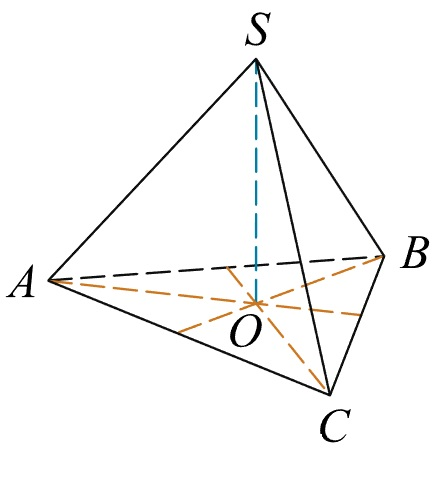
\includegraphics[align=t, width=\linewidth]{\picpath/G111M6L1-1}
		\end{minipage}
		\item В правильной четырехугольной пирамиде \(SABCD\) точка \(O\) --- центр основания, \(S\) --- вершина, \(SO=15, BD=16\). Найдите боковое ребро \(SA\).
		\item Объем параллелепипеда \(ABCDA_1B_1C_1D_1\) равен \(9\). Найдите объем треугольной пирамиды \(ABCA_1\).
		\item Во сколько раз увеличится объем правильного тетраэдра, если все его ребра увеличить в два раза?
		\item Первая цилиндрическая кружка вдвое выше второй, зато вторая в полтора раза шире. Найдите отношение объема второй кружки к объему первой. (Задание из пробника, вариант \( 1 \)).
		\item Сторона основания правильной шестиугольной пирамиды равна \( 3 \), боковое ребро равно \( 6 \).	Найдите объем пирамиды. (Задание из пробника, вариант \( 2 \)).
		\item Объём треугольной призмы, отсекаемой от куба плоскостью, проходящей через середины двух рёбер, выходящих из одной вершины, и параллельной третьему ребру, выходящему из	этой же вершины, равен \( 4 \). Найдите объём куба. (Задание из пробника, вариант \( 3 \)).
		\item Решите уравнения:
		\begin{tasks}(2)
			\task \( \sin x=\dfrac{1}{2} \)
			\task \( \cos x=-\dfrac{\sqrt{3}}{2} \)
			\task \( \sin x = -\dfrac{\sqrt{2}}{2} \)
			\task \( \tg x = \dfrac{-\sqrt{3}}{3} \)
			\task \( \ctg x = -1 \)
			\task \( \cos x = \dfrac{\sqrt{2}}{2} \)
		\end{tasks}
		\item Решить уравнения:
		\begin{tasks}(2)
			\task \( \cos\left( 2x+\dfrac{\pi}{4} \right)=\dfrac{\sqrt{2}}{2} \)
			\task \( \sin \left( 2x-\dfrac{3\pi}{2} \right) = -1 \)
			\task \( \cos \left( \dfrac{\pi}{4}-x \right)=\dfrac{\sqrt{3}}{2} \)
			\task \( \ctg\left( 2x-\dfrac{3\pi}{4} \right)=-1 \)
		\end{tasks}
	\end{listofex}
\end{class}
%END_FOLD

%BEGIN_FOLD % ====>>_____ Занятие 2 _____<<====
\begin{class}[number=2]
	\begin{listofex}
		\item Объём треугольной призмы, отсекаемой от куба плоскостью, проходящей через середины двух рёбер, выходящих из одной вершины, и параллельной третьему ребру, выходящему из	этой же вершины, равен \( 4 \). Найдите объём куба. (Задание из пробника, вариант \( 3 \)).
		\item 
		\begin{minipage}[t]{\bodywidth}
			На рисунке изображен многогранник, все двугранные углы многогранника прямые. Найдите квадрат расстояния между вершинами \(B_2\) и \(D_3\) .
		\end{minipage}
		\hspace{0.02\linewidth}
		\begin{minipage}[t]{\picwidth}
			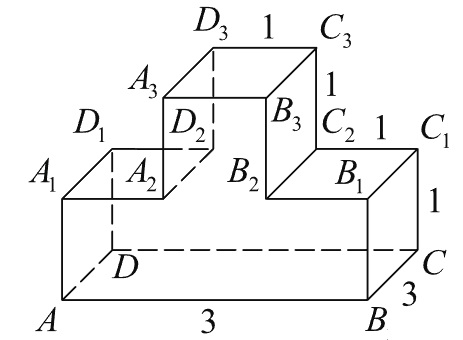
\includegraphics[align=t, width=\linewidth]{\picpath/G101M5L6-2}
		\end{minipage}
		\item С помощью этого же рисунка найдите:
		\begin{tasks}(1)
			\task расстояние между вершинами \(B\) и \(D_2\),
			\task тангенс угла \(C_2C_3B_2\).
		\end{tasks}
		\item 
		\begin{minipage}[t]{\bodywidth}
			На рисунке изображен многогранник, все двугранные углы многогранника прямые. Найдите его объём и площадь поверхности.
		\end{minipage}
		\hspace{0.02\linewidth}
		\begin{minipage}[t]{\picwidth}
			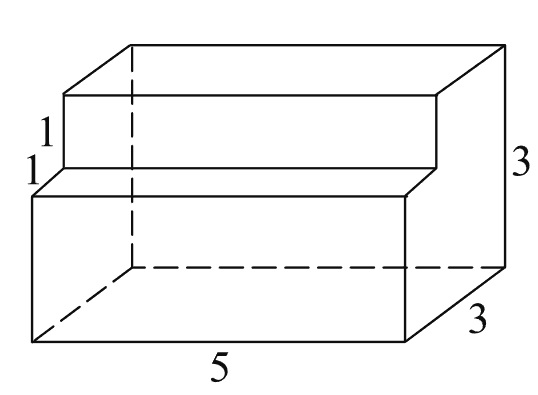
\includegraphics[align=t, width=\linewidth]{\picpath/G101M5L7-2}
		\end{minipage}
		\item 
		\begin{minipage}[t]{\bodywidth}
			На рисунке изображен многогранник, все двугранные углы многогранника прямые. Найдите его объём и площадь поверхности.
		\end{minipage}
		\hspace{0.02\linewidth}
		\begin{minipage}[t]{\picwidth}
			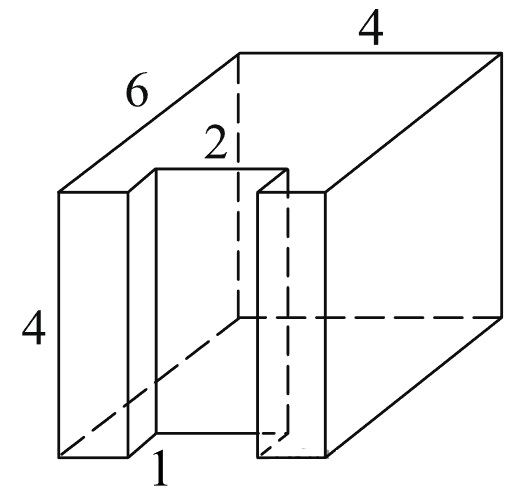
\includegraphics[align=t, width=\linewidth]{\picpath/G102M5L7-2}
		\end{minipage}
		\item 
		\begin{minipage}[t]{\bodywidth}
			На рисунке изображён многогранник, все двугранные углы многогранника прямые. Найдите расстояние между вершинами \(A\) и \(C_2\) .
		\end{minipage}
		\hspace{0.02\linewidth}
		\begin{minipage}[t]{\picwidth}
			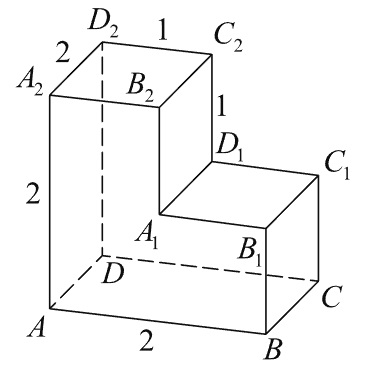
\includegraphics[align=t, width=\linewidth]{\picpath/G101M5L6-1}
		\end{minipage}
			\item В цилиндрический сосуд налили \(2000\) см\(^3\) воды. Уровень воды при этом достигает высоты \(12\) см. В жидкость полностью погрузили деталь. При этом уровень жидкости в сосуде поднялся на \(9\) см. Чему равен объем детали? Ответ выразите в см\(^3\).
		\item В цилиндрическом сосуде уровень жидкости достигает \(16\) см. На какой высоте будет находиться уровень жидкости, если ее перелить во второй сосуд, диаметр которого в \(2\) раза больше первого? Ответ дайте в сантиметрах.
		\item Объем первого цилиндра равен \(12\) м\(^3\). У второго цилиндра высота в три раза больше, а радиус основания --- в два раза меньше, чем у первого. Найдите объем второго цилиндра. Ответ дайте в кубических метрах.
		\item Объем конуса равен \(16\). Через середину высоты параллельно основанию конуса проведено сечение, которое является основанием меньшего конуса с той же вершиной. Найдите объем меньшего конуса.
		\item Во сколько раз уменьшится объем конуса, если его высота уменьшится в \(3\) раза, а радиус основания останется прежним?
		\item Диаметр основания конуса равен \(6\), а угол при вершине осевого сечения равен \(90\pi \). Вычислите объем конуса, деленный на \( \pi \).
		\item Решите уравнения:
		\begin{tasks}(2)
			\task \( \sin x=\dfrac{1}{2} \)
			\task \( \cos x=-\dfrac{\sqrt{3}}{2} \)
			\task \( \sin x = -\dfrac{\sqrt{2}}{2} \)
			\task \( \tg x = \dfrac{-\sqrt{3}}{3} \)
			\task \( \ctg x = -1 \)
			\task \( \cos x = \dfrac{\sqrt{2}}{2} \)
		\end{tasks}
		\item Решить уравнения:
		\begin{tasks}(2)
			\task \( \cos\left( 2x+\dfrac{\pi}{4} \right)=\dfrac{\sqrt{2}}{2} \)
			\task \( \sin \left( 2x-\dfrac{3\pi}{2} \right) = -1 \)
			\task \( \cos \left( \dfrac{\pi}{4}-x \right)=\dfrac{\sqrt{3}}{2} \)
			\task \( \ctg\left( 2x-\dfrac{3\pi}{4} \right)=-1 \)
		\end{tasks}
	\end{listofex}
\end{class}
%END_FOLD

%BEGIN_FOLD % ====>>_ Домашняя работа 1 _<<====
\begin{homework}[number=1]
	\begin{listofex}
		\item Объем прямоугольного параллелепипеда равен \(24\). Одно из его ребер равно \(3\). Найдите площадь грани параллелепипеда, перпендикулярной этому ребру.
		\item 
		\begin{minipage}[t]{\bodywidth}
			В правильной треугольной пирамиде \(SABC\) точка \(M\) --- середина ребра \(AB\), \(S\) --- вершина. Известно, что \(BC = 3\), а площадь боковой поверхности пирамиды равна \(45\). Найдите длину отрезка \(SM\).
		\end{minipage}
		\hspace{0.02\linewidth}
		\begin{minipage}[t]{\picwidth}
			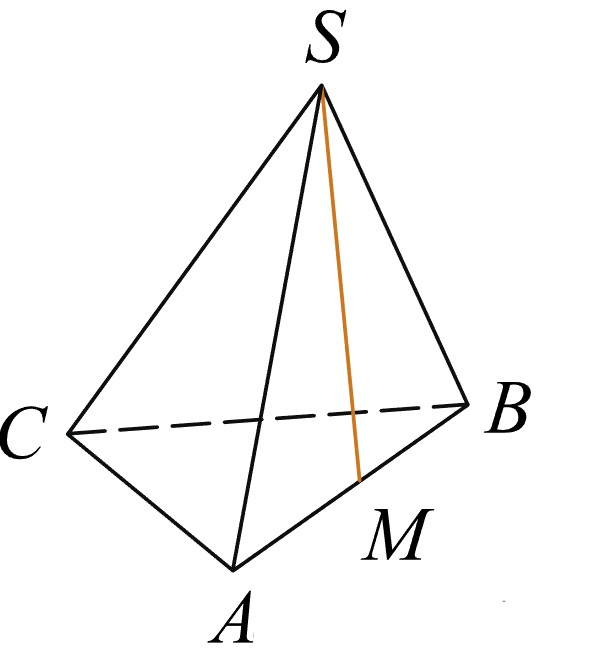
\includegraphics[align=t, width=\linewidth]{\picpath/G111M6L1-2}
		\end{minipage}
		\item 
		\begin{minipage}[t]{\bodywidth}
			На рисунке изображен многогранник, все двугранные углы многогранника прямые. Найдите его объём и площадь поверхности.
		\end{minipage}
		\hspace{0.02\linewidth}
		\begin{minipage}[t]{\picwidth}
			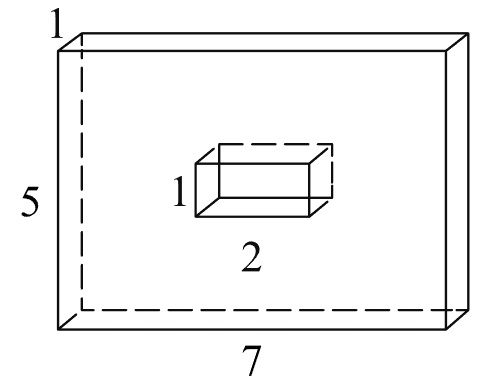
\includegraphics[align=t, width=\linewidth]{\picpath/G102M5L7-3}
		\end{minipage}
		\item 
		\begin{minipage}[t]{\bodywidth}
			На рисунке изображен многогранник, все двугранные углы многогранника прямые. Найдите его объём и площадь поверхности.
		\end{minipage}
		\hspace{0.02\linewidth}
		\begin{minipage}[t]{\picwidth}
			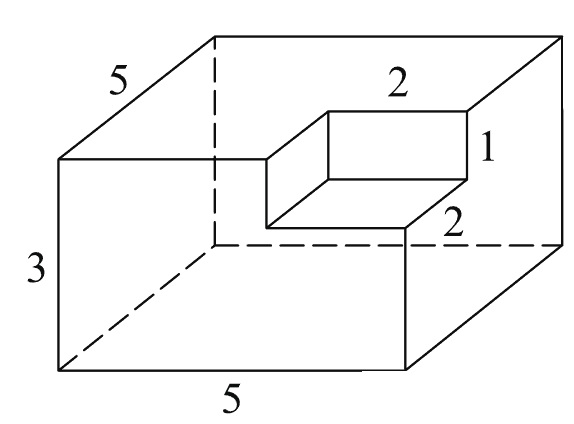
\includegraphics[align=t, width=\linewidth]{\picpath/G101M5L7-3}
		\end{minipage}
		\item Два ребра прямоугольного параллелепипеда, выходящие из одной вершины, равны \( 1 \), \( 2 \). Площадь поверхности параллелепипеда равна \( 16 \). Найдите его диагональ.
		\item Площадь грани прямоугольного параллелепипеда равна \( 12 \). Ребро, перпендикулярное этой грани, равно 4. Найдите объем параллелепипеда.
		\item Диагональ куба равна \( 4 \). Найдите площадь его поверхности.
		\item Ребра прямоугольного параллелепипеда равны \( 7 \), \( 12 \) и \( 5 \). Найдите объем и площадь поверхности этого параллелепипеда.
		\item В правильной треугольной пирамиде \(SABC\) медианы основания \(ABC\) пересекаются в точке \(O\). Площадь треугольника \(ABC\) равна \(9\); объем пирамиды равен \(6\). Найдите длину отрезка \(OS\).
		\newpage
		\item Решите уравнения:
		\begin{tasks}(2)
			\task \( \log_{1/7}(7-x)=-2\)
			\task \( \log_4(16+x)=\log_23 \)
			\task \( \log_4(4-x)=2\log_25 \)
			\task \( \log_5(x^2+2x)=\log_5(x^2+10) \)
		\end{tasks}
		\item Решите уравнение:
		\begin{tasks}(2)
			\task \( \dfrac{13x}{2x^2-7}=1 \)
			\task \( \dfrac{1}{9x-7}=\dfrac{1}{2} \)
			\task \( \sqrt[3]{\dfrac{1}{10x+6}}=1 \)
			\task \( \dfrac{x+89}{x-7}=\dfrac{-5}{x-7} \)
		\end{tasks}
		\item Найдите \( \cos x\), если \( \sin x=-0,6 \) при \( \dfrac{3\pi}{2}<x<2\pi \)
	\end{listofex}
\end{homework}
%END_FOLD

%BEGIN_FOLD % ====>>_____ Занятие 3 _____<<====
\begin{class}[number=3]
	\title{Самостоятельное прорешивание (30 минут)}
	\begin{listofex}
		\item Боковая сторона равнобедренного треугольника равна \( 7 \), угол при вершине, противолежащей основанию, равен \( 120\degree \). Найдите диаметр описанной окружности этого треугольника.
		\item Объем параллелепипеда \( ABCDA_1B_1C_1D_1 \) равен \( 9 \). Найдите объем треугольной пирамиды \( ABCA_1 \).
		\item На изготовление \( 99 \) деталей первый рабочий тратит на \( 2 \) часа меньше, чем второй рабочий на изготовление \( 110 \) таких же деталей. Известно, что первый рабочий за час делает на \( 1 \) деталь больше, чем второй. Сколько деталей в час делает второй рабочий?
		\item Фабрика выпускает сумки. В среднем на \( 190 \) качественных сумок приходится восемь сумок со скрытыми дефектами. Найдите вероятность того, что купленная сумка окажется качественной. Результат округлите до сотых.
		\item Вероятность того, что батарейка бракованная, равна \( 0,06 \). Покупатель в магазине выбирает случайную упаковку, в которой две таких батарейки. Найдите вероятность того, что обе батарейки окажутся исправными.
		\item На рисунке изображён график функции вида \( f(x)=\dfrac{x^2}{a}+bx+c \),  где числа \( a \), \( b \) и \( c \) --- целые. Найдите значение \( f(4) \).
		\begin{center}
			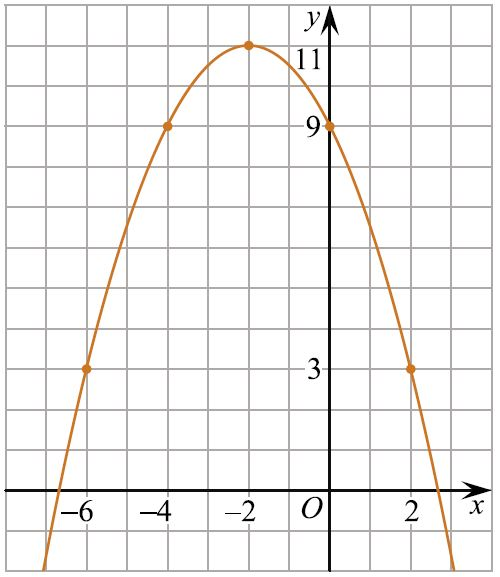
\includegraphics[align=t, width=0.4\linewidth]{\picpath/G112M3C2-4}
		\end{center}
	\end{listofex}
	\newpage
	\title{Основная часть занятия}
	\begin{listofex}
		\item Решите уравнения:
		\begin{tasks}(2)
			\task \( \sin x=\dfrac{1}{2} \)
			\task \( \cos x=-\dfrac{\sqrt{3}}{2} \)
			\task \( \sin x = -\dfrac{\sqrt{2}}{2} \)
			\task \( \tg x = \dfrac{-\sqrt{3}}{3} \)
			\task \( \ctg^2 x = -1 \)
			\task \( \cos^2 x = \dfrac{1}{2} \)
		\end{tasks}
		\item Решить уравнение \( \cos\dfrac{\pi(x-7)}{3}=\dfrac{1}{2} \). В ответ запишите наибольший отрицательный корень.
		\item Решить уравнение \( \tg\dfrac{\pi x}{4}=\dfrac{1}{2} \). В ответ запишите наибольший отрицательный корень.
		\item Решить уравнение \( \cos\dfrac{\pi(x-4)}{2}=\dfrac{3}{2} \). В ответ запишите наибольший отрицательный корень.
		\item Решить уравнение \( \sin\dfrac{2\pi x}{3}=\dfrac{1}{2} \). В ответ запишите наибольший отрицательный корень.
		\item Решить уравнение \( \cos\dfrac{\pi(3x+6)}{3}=\dfrac{\sqrt{2}}{2} \). В ответ запишите наименьший положительный корень.
	\end{listofex}
\end{class}
%END_FOLD

%BEGIN_FOLD % ====>>_____ Занятие 4 _____<<====
\begin{class}[number=4]
	\begin{listofex}
		\item Решить уравнение \( \tg\dfrac{\pi x}{4}=\dfrac{1}{2} \). В ответ запишите наибольший отрицательный корень.
		\item Решить уравнение \( \cos\dfrac{\pi(x-4)}{2}=\dfrac{\sqrt{3}}{2} \). В ответ запишите наибольший отрицательный корень.
		\item Решить уравнение \( \sin\dfrac{2\pi x}{3}=\dfrac{1}{2} \). В ответ запишите наибольший отрицательный корень.
		\item Решить уравнение \( \cos\dfrac{\pi(3x+6)}{3}=\dfrac{\sqrt{2}}{2} \). В ответ запишите наименьший положительный корень.
		\item Решите уравнения:
		\begin{tasks}(2)
			\task \( \sin \left( x+\dfrac{\pi}{4} \right) = \dfrac{1}{2} \)
			\task \( \tg \left( 3x-\dfrac{12\pi}{7} \right) = -1 \)
			\task \( \cos \left( \dfrac{5\pi}{8}+x \right) = \dfrac{\sqrt{2}}{2} \)
		\end{tasks}
		\item Решите уравнение \( \sin^2x-\sin x=0 \)
		\item Решите уравнение \( 5\tg^2x+6\tg x+1=0 \)
		\item Решите уравнение \( \cos^2x=\dfrac{1}{4} \)
		\item  Решите уравнение \( \tg x-2\ctg x=1 \)
		\item Найдите точку максимума функции \( y=-\dfrac{x^2+225}{x} \)
		\item Найдите точку минимума функции \( y=\dfrac{400}{x}+x+7 \)
		\item Найдите точку максимума функции \( y=(x+16)e^{16-x} \)
		\item Найдите наибольшее значение функции \( y=(x-9)e^{10-x} \) на отрезке \( [-11;11] \)
		\item
		\begin{minipage}[t]{0.43\textwidth}
			На рисунке изображён график функции вида \(f(x)=ax-|bx+c|+d\), где числа \(a, b, c, d\) --- целые. Найдите корень уравнения \(ax=d\).
		\end{minipage}
		\begin{minipage}[c]{0.1\textwidth}
			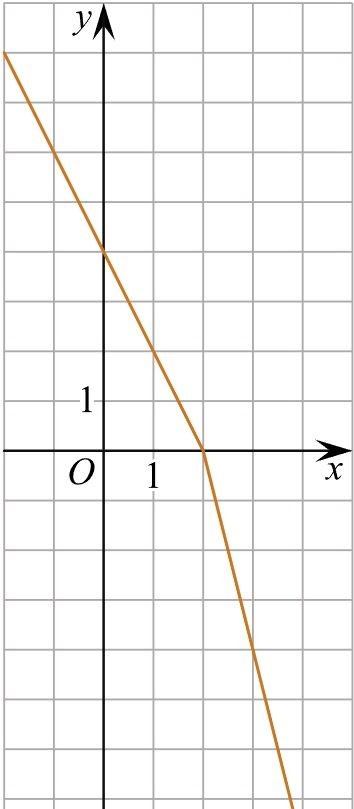
\includegraphics[align=t, width=\textwidth]{../pics/G101M4H2-7.jpg}
		\end{minipage}
	\end{listofex}
\end{class}
%END_FOLD

%BEGIN_FOLD % ====>>_ Домашняя работа 2 _<<====
\begin{homework}[number=2]
	\begin{listofex}
		\item Решить уравнение \( \sin\dfrac{\pi(4x-3)}{4}=1 \). В ответ запишите наибольший отрицательный корень.
		\item Решить уравнение \( \sin\dfrac{\pi(8x+3)}{6}=0,5 \). В ответ запишите наименьший положительный корень.
		\item Решить уравнение \( \cos\dfrac{\pi(x+1)}{4}=\dfrac{\sqrt{2}}{2} \). В ответ запишите наибольший отрицательный корень.
		\item Решить уравнение \( \cos\dfrac{\pi(4x+1)}{6}=\dfrac{\sqrt{3}}{2} \). В ответ запишите наибольший отрицательный корень.
		\item Решить уравнение \( \tg\dfrac{\pi(x-3)}{6}=\dfrac{1}{\sqrt{3}} \). В ответ запишите наибольший отрицательный корень.
		\item Решить уравнение \( \tg\dfrac{\pi(4x-5)}{4}=-1 \). В ответ запишите наименьший положительный корень.
		\item Заказ на \(156\) деталей первый рабочий выполняет на \(1\) час быстрее, чем второй. Сколько деталей за час изготавливает первый рабочий, если известно, что он за час изготавливает на \(1\) деталь больше второго?
		\item
		\begin{minipage}[t]{\bodywidth}
			На рисунке изображён график функции вида \[ f(x)=ax+|bx+c|+d, \] где числа \(a, b, c, d\) --- целые. Найдите корень уравнения \(ax+d=-15\).
		\end{minipage}
		\hspace{0.02\linewidth}
		\begin{minipage}[t]{\picwidth}
			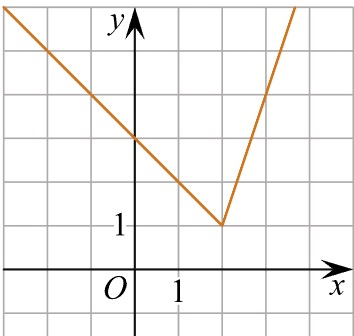
\includegraphics[align=t, width=\linewidth]{\picpath/G101M4C5-7}
		\end{minipage}
	\end{listofex}
\end{homework}
%END_FOLD

%BEGIN_FOLD % ====>>_____ Занятие 5 _____<<====
\begin{class}[number=5]
	\begin{listofex}
		\item Решите уравнения:
		\begin{tasks}(2)
			\task \( 6\cos^2{x}+\cos{x}-1=0 \)
			\task \( 2\cos^2{3x}-5\cos{3x}-3=0 \)
			\task \( 2\cos^2{\dfrac{x}{3}}+3\cos{\dfrac{x}{3}}-2=0 \)
			%\task \( 2\sin^2x+3\cos{x}=0 \)
			\task \( 8\sin^2{2x}+\cos{2x}+1=0 \)
			%\task \( 5\cos^2{2x}+6\sin{2x}-6=0 \) V DZ
			%\task \( 4\sin{3x}+\cos^2{3x}=4 \) V DZ
			%\task \( 3\tg^2{x}+2\tg{x}-1=0 \) V DZ
			\task \( \ctg^2{2x}-6\ctg{2x}+5=0 \)
		\end{tasks}
		\item Решите уравнения:
		\begin{tasks}(1)
			\task \( \sin{2x}+2\sin{(-x)}+\cos{(-x)}-1=0 \)
			\task \( \cos{2x}+\sqrt{2}\cos{\left( \dfrac{\pi}{2}-x \right)}-1=0 \)
			\task \( 7\sin{ \left( \dfrac{\pi}{2}+x \right) +4\sqrt{3}\sin{x} \cos{x} = 4 \cos^3{x}  } \)
			%\task \( \cos{2x}=1-\cos{\left( \dfrac{\pi}{2}-x \right) } \)
			\task \( \sin{(\pi-x)}- \cos{\left( \dfrac{\pi}{2}+x \right) = -1 }  \)
		\end{tasks}
	\end{listofex}
\end{class}
%END_FOLD

%BEGIN_FOLD % ====>>_____ Занятие 6 _____<<====
\begin{class}[number=6]
	\begin{listofex}
		\item Занятие 6
	\end{listofex}
\end{class}
%END_FOLD

%BEGIN_FOLD % ====>>_ Домашняя работа 3 _<<====
\begin{homework}[number=3]
	\begin{listofex}
		\item Решите уравнения:
		\begin{tasks}(1)
			\task \( 2\sin^2x+3\cos{x}=0 \)
			\task \( 5\cos^2{2x}+6\sin{2x}-6=0 \)
			\task \( 4\sin{3x}+\cos^2{3x}=4 \)
			\task \( 3\tg^2{x}+2\tg{x}-1=0 \)
			%\task \( 2x\cos{x}-8\cos{x}+x-4=0 \)
			%\task \( 2\sin{(\pi+x)}\cdot \sin{0,5\pi+x}=\sin{x} \)
		\end{tasks}
		\item Решите уравнения:
		\begin{tasks}(1)
			\task \( 2\sin{2x}=4\cos{x}-\sin{x}+1 \)
			\task \( \sin{2x}+\sqrt{2}\sin{x}=2\cos{x}+\sqrt{2} \)
			\task \( \cos^2{x}-\dfrac{1}{2} \cdot \sin{2x} + \cos{x} = \sin{x} \)
		\end{tasks}
		\item Решите уравнения:
		\begin{tasks}
			\task \( \cos{\left( \dfrac{\pi}{2}+2x \right)} = \sqrt{2} \sin{x} \)
			\task \( 2\sin{ \left( \dfrac{7\pi}{2}-x \right)} \sin{x}=\cos{x} \)
		\end{tasks}
	\end{listofex}
\end{homework}
%END_FOLD

%BEGIN_FOLD % ====>>_____ Занятие 7 _____<<====
\begin{class}[number=7]
	\begin{listofex}
		\item
		а) Решите уравнение: \( 3\sqrt{3} \cos{\left( \dfrac{3\pi}{2} + x \right)} -3=2\sin^2{x}  \),\\[0.5em]
		б) Найдите корни на промежутке: \( \left[ -\dfrac{3\pi}{2}; 0 \right] \).
		\item
		а) Решите уравнение: \( \cos^2{x}+\cos^2{\dfrac{\pi}{6}} = \cos^2{2x} + \sin^2{\dfrac{\pi}{3}} \),\\[0.5em]
		б) Найдите корни на промежутке: \( \left[ 2\pi; \dfrac{7\pi}{2} \right] \).
		\item
		а) Решите уравнение:
		\( 8 \sin{x}+4\cos^2{x}=7 \),\\[0.5em]
		б) Найдите корни на промежутке:
		\( \left[ -\dfrac{3\pi}{2}; -\dfrac{\pi}{2} \right] \).
		\item
		а) Решите уравнение:
		\( 2 \cos^2{x} + 19 \sin{x}+8=0 \),\\[0.5em]
		б) Найдите корни на промежутке:
		\( \left[ -\pi; \dfrac{\pi}{2} \right] \).
		\item
		а) Решите уравнение:
		\( 2\sin x+2\cos\left( 2x-\dfrac{\pi}{4} \right)=\sqrt{2}\sin2x-\dfrac{1}{\sqrt{2}} \),\\[0.5em]
		б) Найдите корни на промежутке:
		\( \left[ 5\pi; \dfrac{13\pi}{2} \right] \).
		\item
		а) Решите уравнение:
		\( 4\sin\left( x-\dfrac{7\pi}{2} \right)=\dfrac{3}{\cos x} \),\\[0.5em]
		б) Найдите корни на промежутке:
		\( \left[ -3\pi; -\dfrac{3\pi}{2} \right] \).
		\item
		а) Решите уравнение:
		\( \dfrac{7}{1-\cos^2 x}+\dfrac{9}{\sin x}=10 \),\\[0.5em]
		б) Найдите корни на промежутке:
		\( \left[ -2\pi;-\dfrac{\pi}{2} \right] \).
	\end{listofex}
\end{class}
%END_FOLD

%BEGIN_FOLD % ====>>_ Проверочная работа _<<====
\begin{exam}
	\begin{listofex}
		\item Занятие 8
	\end{listofex}
\end{exam}
%END_FOLD

%BEGIN_FOLD % ====>>_ Консультация _<<====
\begin{consultation}
	\begin{listofex}
		\item Найдите наибольшее значение функции \( y=\dfrac{x^2+25}{x} \) на отрезке \( [-12;-1] \).
		\item Найдите наибольшее значение функции \( y=(x^2-3x+3)\cdot e^{3-x} \) на отрезке \( [2;5] \).
		\item Найдите наименьшее значение функции \( y=2^{x^2+2x+5} \)
		\item Найдитe точку минимума функции \( y=\sqrt{x^2-6x+11} \).
		\item Найдите точку максимума функции \( y=\log_2(2+2x-x^2)-2 \).
		\item Найдите наибольшее значение функции \( y=\ln(8x)-8x+7 \) на отрезке \( \left[ \dfrac{1}{16};\dfrac{5}{16} \right] \).
		\item Найдите наибольше значение функции \( y=20\tg x-20x+5\pi-6 \) на отрезке \( 	\left[-\dfrac{\pi}{4}; \dfrac{\pi}{4}\right] \).
		\item Найдите точку минимума функции \( y=(1-2x)\cos x+2\sin x+7 \), принадлежащую промежутку \( \left( 0;\dfrac{\pi}{2} \right) \).
		\item Найдите наибольшее значение функции \( y=99x-97\sin x+62 \) на отрезке \( \left[-\dfrac{\pi}{2};0\right] \).
	\end{listofex}
	\newpage
	\title{Домашняя работа}
	\begin{listofex}
		\item Найдите точку минимумы функции \( y=\log_5(x^2-6x+12)+2 \).
		\item Найдите точку максимума функции \( y=\sqrt{4-4x-x^2} \).
		\item Найдите наибольшее значение функции \( y=3^{-7-6x-x^2} \).
		\item Найдите наименьшее значение функции \( y=69\cos x+71x+48 \) на отрезке \( \left[0;\dfrac{3\pi}{2}\right] \).
	\end{listofex}
\end{consultation}
%END_FOLD

%BEGIN_FOLD % ====>>_ Консультация _<<====
\begin{consultation}
	\title{Номер 3}
	\begin{listofex}
		\item Фабрика выпускает сумки. В среднем на \( 160 \) качественных сумок приходится две сумки со скрытыми дефектами. Найдите вероятность того, что купленная сумка окажется качественной. Результат округлите до сотых.
		\item На рок-фестивале выступают группы  — по одной от каждой из заявленных стран. Порядок выступления определяется жребием. Какова вероятность того, что группа из Китая будет выступать после группы из Вьетнама и после группы из Канады? Результат округлите до сотых.
		\item В некотором городе из \( 5000 \) появившихся на свет младенцев \( 2440 \) девочек. Найдите частоту рождения мальчиков в этом городе. Результат округлите до тысячных.
		\item За круглый стол на \( 9 \) стульев в случайном порядке рассаживаются \( 7 \) мальчиков и \( 2 \) девочки. Найдите вероятность того, что девочки не будут сидеть рядом.
		\item В случайном эксперименте симметричную монету бросают дважды. Найдите вероятность того, что наступит исход ОР (в первый раз выпадает орёл, во второй --- решка).
	\end{listofex}
	\title{Номер 4}
	\begin{listofex}[resume]
		\item Если шахматист А. играет белыми фигурами, то он выигрывает у шахматиста Б. с вероятностью \( 0,5 \). Если А. играет черными, то А. выигрывает у Б. с вероятностью \( 0,34 \). Шахматисты А. и Б. играют две партии, причём во второй партии меняют цвет фигур. Найдите вероятность того, что А. выиграет оба раза.
		\item Биатлонист пять раз стреляет по мишеням. Вероятность попадания в мишень при одном выстреле равна \( 0,8 \). Найдите вероятность того, что биатлонист первые три раза попал в мишени, а последние два промахнулся. Результат округлите до сотых.
		\item При артиллерийской стрельбе автоматическая система делает выстрел по цели. Если цель не уничтожена, то система делает повторный выстрел. Выстрелы повторяются до тех пор, пока цель не будет уничтожена. Вероятность уничтожения некоторой цели при первом выстреле равна \( 0,4 \), а при каждом последующем --- \( 0,6 \). Сколько выстрелов потребуется для того, чтобы вероятность уничтожения цели была не менее \( 0,98 \)?
		\item В Волшебной стране бывает два типа погоды: хорошая и отличная, причём погода, установившись утром, держится неизменной весь день. Известно, что с вероятностью \( 0,8 \) погода завтра будет такой же, как и сегодня. Сегодня \( 3 \) июля, погода в Волшебной стране хорошая. Найдите вероятность того, что \( 6 \) июля в Волшебной стране будет отличная погода.
		\item Ковбой Джон попадает в муху на стене с вероятностью \( 0,9 \), если стреляет из пристрелянного револьвера. Если Джон стреляет из непристрелянного револьвера, то он попадает в муху с вероятностью \( 0,2 \). На столе лежит \( 10 \) револьверов, из них только \( 4 \) пристрелянные. Ковбой Джон видит на стене муху, наудачу хватает первый попавшийся револьвер и стреляет в муху. Найдите вероятность того, что Джон промахнётся.
	\end{listofex}
	\title{Номер 8}
	\begin{listofex}[resume]
		\item При движении ракеты еe видимая для неподвижного наблюдателя длина, измеряемая в метрах, сокращается по закону \( l=l_0\sqrt{1-\dfrac{v^2}{c^2}} \),  где \( l_0 = 5 \) м  --- длина покоящейся ракеты, \( c=3\cdot10^5   \) км/с --- скорость света, а  \( v \) --- скорость ракеты (в км/с). Какова должна быть минимальная скорость ракеты, чтобы еe наблюдаемая длина стала не более \( 4 \) м? Ответ выразите в км/с.
		\item По закону Ома для полной цепи сила тока, измеряемая в амперах, равна \( I=\dfrac{\epsilon}{R+r} \),  где \( \epsilon \) --- ЭДС источника (в вольтах), \( r=1 \) Ом --- его внутреннее сопротивление, \( R \) --- сопротивление цепи (в омах). При каком наименьшем сопротивлении цепи сила тока будет составлять не более \( 20\% \) от силы тока короткого замыкания \( I \)кз\( =\dfrac{\epsilon}{r} \)? (Ответ выразите в омах.)
	\end{listofex}
		\title{Номер 9}
	\begin{listofex}[resume]
		\item Имеются два сосуда. Первый содержит \( 30 \) кг, а второй --- \( 20 \) кг раствора кислоты различной концентрации. Если эти растворы смешать, то получится раствор, содержащий \( 68\% \) кислоты. Если же смешать равные массы этих растворов, то получится раствор, содержащий \( 70\% \) кислоты. Сколько килограммов кислоты содержится в первом сосуде?
		\item Имеется два сплава. Первый содержит \( 15\% \) никеля, второй --- \( 35\% \) никеля. Из этих двух сплавов получили третий сплав массой \( 140 \) кг, содержащий \( 30\% \) никеля. На сколько килограммов масса первого сплава была меньше массы второго?
	\end{listofex}
\end{consultation}
%END_FOLD